%======================================================================
% PD-RobustBench manuscript
% Compile: pdflatex main && bibtex main (or use the embedded thebibliography)
%======================================================================
\documentclass[11pt,a4paper]{article}
\usepackage[margin=2.4cm]{geometry}
\usepackage{graphicx}
\usepackage{booktabs}
\usepackage{amsmath}
\usepackage{multirow}
\usepackage[hidelinks]{hyperref}
\usepackage{xcolor}
\usepackage{caption}
\captionsetup{font=small,labelfont=bf}

\title{\textbf{PD-RobustBench: A Corruption-Robustness and Explainability Framework for Parkinson's Disease Detection from Hand-Drawn Images}}

\author{Ramtin Torik \and Iman Abedini \and Kimia Peyvandi%
\thanks{Corresponding author: Kimia Peyvandi, \texttt{kpeyvandi@semnan.ac.ir}}\\[4pt]
\small [Department], Semnan University, Semnan, Iran\\
\small Ramtin Torik: \texttt{ramtin.torik82@gmail.com}; Iman Abedini: \texttt{imanabedini.ai@gmail.com}}
\date{}

\begin{document}
\maketitle

\begin{abstract}
Deep learning models detect Parkinson's disease (PD) from hand-drawn spiral,
wave, and meander images with high reported accuracy, yet these figures are
obtained on clean data, while deployed models face compression, blur, noise,
and imperfect acquisition. We present PD-RobustBench, a reproducible
framework that evaluates PD-detection models under eight acquisition-inspired
corruptions at five severity levels, following the ImageNet-C methodology,
and additionally measures how the models' Grad-CAM explanations change under
the same corruptions. Prediction and explanation degradation are combined
into a Parkinson Robustness Score (PRS, 0--100). Four ImageNet-pretrained
backbones (ResNet50, VGG16, EfficientNet-B0, MobileNetV3-Large) are adapted
with light head training on two public datasets (Parkinson's Drawings and
HandPD), yielding sixteen configurations that are evaluated across 41
conditions and three random seeds. Rotation is the most damaging corruption
(balanced-accuracy loss of 10--22\%), whereas contrast is nearly harmless.
Grad-CAM maps decorrelate strongly at high severity (Spearman $\rho=0.29$
under rotation), so explanations can drift while predictions survive. PRS
separates backbones (82--96) with explicitly reported seed and weight
sensitivity. The framework supports standardized, explainability-aware
robustness reporting and is intended for methodological benchmarking rather
than clinical validation.
\end{abstract}

\noindent\textbf{Keywords:} Parkinson's disease; handwriting analysis;
corruption robustness; benchmark; Grad-CAM; explainable AI; transfer learning

\section{Introduction}
Parkinson's disease (PD) is among the fastest-growing neurodegenerative
disorders, and its motor symptoms alter fine motor control long before a
clinical diagnosis is established. Handwriting and drawing tasks -- most
prominently tracing a spiral or a wave, or drawing meanders -- are inexpensive,
non-invasive markers of these motor deficits
\cite{zham2016,zham2017,pereira2016}. A growing literature therefore trains
deep neural networks to classify such images as PD or healthy, with reported
test accuracies frequently exceeding 90\%
\cite{huang2024,frontiers2024,aims2024,diagnostics2025}.

These headline numbers, however, share a common weakness: they are measured
once, on clean test images, under a single acquisition pipeline. Real
deployments inherit far more varied imaging conditions. A photograph of a
paper drawing may be saved with aggressive JPEG compression; scans may be
slightly out of focus or noisy; lighting changes brightness and contrast; and
paper is rarely aligned perfectly with the camera. If a model's accuracy or
its \emph{explanations} collapse under such mundane degradations, then its
clean-data accuracy is a poor guide to clinical usefulness. This concern is
well recognized in the broader computer-vision and medical-imaging literature
\cite{hendrycks2019,javed2024,boone2023}, where corruption benchmarks such as
ImageNet-C \cite{hendrycks2019} and MedMNIST-C have become standard tools --
but, to the best of our knowledge, no such systematic robustness evaluation
has been applied to PD detection from drawings.

We address this gap with \textbf{PD-RobustBench}, a framework that:
(i) evaluates a candidate CNN-based PD-detection model under \emph{eight
synthetic, acquisition-inspired corruption families at five severity levels}
(40 corrupted conditions per model), adapted
from ImageNet-C to black-ink-on-white drawing images;
(ii) reports the full metric suite (accuracy, balanced accuracy, precision,
sensitivity, specificity, F1, ROC-AUC) for every condition rather than a
single number;
(iii) tracks \emph{explanation stability} by comparing Grad-CAM maps computed
on corrupted images with those computed on the clean originals (Spearman/Pearson
correlation, SSIM, and IoU of the top-20\% most active pixels); and
(iv) condenses the outcome into a single \emph{Parkinson Robustness Score}
(PRS, 0--100) that ranks models by weighted relative degradation of accuracy,
F1, and XAI stability.

We instantiate the framework with ResNet50, VGG16, EfficientNet-B0, and
MobileNetV3-Large
backbones pretrained on ImageNet (frozen; only a light classification head is
trained), on two public datasets spanning four image types: Parkinson's
Drawings (spiral, wave) and HandPD (spiral, meander). Every configuration is
trained and evaluated with three random seeds, and the PRS weight
sensitivity is analysed explicitly. The contributions are:
\begin{itemize}
\item to the best of our knowledge, among the first systematic
corruption-robustness benchmarks for image-based PD detection, covering 16
model/dataset configurations $\times$ 41 conditions, three training seeds,
with per-image predictions
released;
\item a quantitative XAI-stability analysis showing how Grad-CAM attention
redistributes under realistic degradations;
\item a compact, interpretable aggregate score (PRS) for model ranking, with
explicit weights, per-corruption breakdowns, and weight/seed sensitivity
analyses; and
\item a fully reproducible open implementation (deterministic corruption
RNG, fixed splits and subsets, cached feature training).
\end{itemize}

Section~\ref{sec:related} reviews related work. Section~\ref{sec:data} describes the datasets and models. Section~\ref{sec:metrics} defines the corruption framework, the evaluation metrics and the PRS. Section~\ref{sec:results} presents the results, and Section~\ref{sec:discussion} discusses practical implications, XAI stability, limitations and conclusions.

\section{Related Work}
\label{sec:related}

\subsection{PD detection from handwriting and drawings}
Table-driven reviews of this niche consistently report high clean accuracies.
On the Parkinson's Drawings dataset (the Kaggle release of the data collected
by Zham et al.\ \cite{zham2016,zham2017}), Huang et al.\
\cite{huang2024} compared VGG16/VGG19, ResNet18/50/101, and a Vision
Transformer, reporting 77--97\% test accuracy depending on architecture,
drawing type, and augmentation strategy, with the wave type consistently
easier than the spiral type. Transfer-learning pipelines reach around
91--95\% \cite{frontiers2024,aims2024,diagnostics2025}. On HandPD
\cite{pereira2016}, classical feature pipelines (e.g., SVM on texture and
kinematic descriptors) established early baselines, and image-level deep
models have since been applied \cite{ml4h2021}. Common to all of these works
is a single clean-test evaluation; none quantifies degradation under image
degradations, which is precisely the dimension our framework adds.

\subsection{Corruption robustness benchmarks}
Hendrycks and Dietterich \cite{hendrycks2019} formalized corruption
robustness evaluation: 15 corruption families at 5 severity levels and the
mean Corruption Error (mCE) as the reference-normalized aggregate.
RobustBench \cite{croce2021} standardized the protocol further. In medical
imaging, MedMNIST-C \cite{medmnistc} applies the same design to twelve
medical classification tasks; ROOD-MRI \cite{boone2023} benchmarks MRI
segmentation under distribution shifts; surveys \cite{javed2024} and
methodological work \cite{shen2025} document consistent accuracy loss under
realistic corruptions and recommend reporting degradation curves rather than
single clean-data scores. Our framework transfers this methodology to
handwriting/drawing images, where degradations correspond to physical
phenomena (out-of-focus scans, compressed uploads, uneven lighting, skewed
paper placement).

\subsection{Explainability and its stability}
Grad-CAM \cite{selvaraju2017} is the de-facto standard for localizing the
image regions driving a CNN decision and has been used qualitatively in the
PD-drawing literature. Adebayo et al.\ \cite{adebayo2018} showed that
saliency maps must be validated rather than trusted blindly, which motivates
treating \emph{explanation stability} as a measurable property: we quantify
how much a model's Grad-CAM map changes when the input is corrupted, using
rank-correlation, SSIM, and top-k IoU. To our knowledge, XAI stability has
not previously been measured for PD detection from drawings.

\section{Datasets and Models}
\label{sec:data}

\subsection{Datasets}
Two public datasets covering four image types are used (examples in
Fig.~\ref{fig:samples}):

\textbf{Parkinson's Drawings (PDRAW).} The Kaggle release
(\cite{kagglepdrawings}) of the spiral/wave data collected by Zham et al.\
\cite{zham2016,zham2017}: 256$\times$256 PNG images, with an official
community split of 72 training and 30 test images per drawing type, balanced
between the healthy and PD classes. We use the released split unchanged.

\textbf{HandPD.} Pereira et al.\ \cite{pereira2016} released scanned
micrographs (~700$\times$700\,px JPG) of spirals and meanders from 92
subjects (74 PD patients, 18 healthy controls; 4 images per subject). HandPD
provides no train/test split, so we create a \emph{subject-wise} stratified
70/30 split (13/5 healthy and 52/22 PD subjects in train/test;
no subject appears in both partitions), yielding 260 training and 108 test
images per drawing type. The class imbalance (4:1 in images) motivates our
use of balanced metrics and a class-balanced training loss.
Table~\ref{tab:split} summarizes both splits. One caveat must be stated
explicitly: the PDRAW release contains no subject identifiers, so
subject-level independence between its train and test partitions cannot be
verified; we flag this as a limitation in Section~\ref{sec:discussion}.

\begin{table}[t]
\centering\small
\caption{Data splits (cells show total, with PD/healthy in parentheses).
The same 92 subjects contribute to both HandPD drawing types. The PDRAW
release does not provide subject identifiers.}
\label{tab:split}
\begin{tabular}{llcccc}
\toprule
Dataset & Type & \multicolumn{2}{c}{Train} & \multicolumn{2}{c}{Test} \\
\cmidrule(lr){3-4}\cmidrule(lr){5-6}
 & & images & subjects & images & subjects \\
\midrule
PDRAW & spiral & 72 (36/36) & n/a & 30 (15/15) & n/a \\
PDRAW & wave & 72 (36/36) & n/a & 30 (15/15) & n/a \\
HandPD & spiral & 260 (208/52) & 65 (52/13) & 108 (88/20) & 27 (22/5) \\
HandPD & meander & 260 (208/52) & 65 (52/13) & 108 (88/20) & 27 (22/5) \\
\bottomrule
\end{tabular}
\end{table}

\begin{figure}[t]
\centering
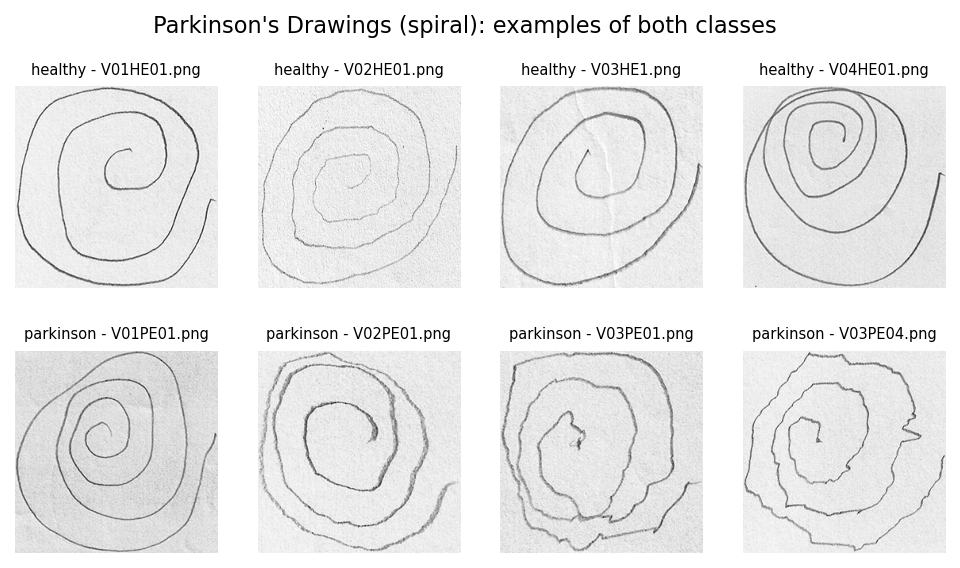
\includegraphics[width=0.85\linewidth]{../../results/figures/fig_dataset_samples.png}
\caption{Examples from the Parkinson's Drawings spiral subset (top: healthy;
bottom: PD). Similar layouts exist for wave (PDRAW) and meander (HandPD).}
\label{fig:samples}
\end{figure}

\subsection{Models}
Four ImageNet-pretrained backbones are evaluated: \textbf{ResNet50}
\cite{resnet}, \textbf{VGG16} \cite{vgg}, \textbf{EfficientNet-B0}
\cite{efficientnet}, and \textbf{MobileNetV3-Large} \cite{mobilenetv3},
chosen because they (a) span several design generations and capacity
classes, (b) are among the most common backbones in this application's
literature, and (c) differ strongly in size and inductive bias, which
matters for robustness.
All models operate on 224$\times$224 RGB inputs with standard ImageNet
normalization. Because ImageNet contains no PD-related class, a minimal
adaptation step is required before any evaluation is possible; we deliberately
keep it as light as possible, in two stages:

\textbf{Stage 1 (head).} The backbone is fully frozen and a uniformly
structured head (global-average-pooled features $\rightarrow$ Dropout(0.3)
$\rightarrow$ Linear(64) $\rightarrow$ ReLU $\rightarrow$ Linear(1)) is
trained with BCEWithLogitsLoss (class-balanced via pos\_weight on the
imbalanced HandPD sets), Adam (lr $10^{-3}$), and early stopping on
validation ROC-AUC (20\% stratified validation split, seed 42). As no
augmentation is used, backbone features are extracted exactly once per
configuration and the head trains on cached features in seconds.

\textbf{Stage 2 (light fine-tune).} Only the final backbone stage
(ResNet50: \texttt{layer4}; VGG16: conv block 5; EfficientNet-B0: the last
three MBConv blocks) is unfrozen and fine-tuned together with the head for at
most 10 epochs (lr $10^{-5}$ backbone / $10^{-4}$ head, early stopping on
validation AUC), leaving the rest of the network untouched. The decision
threshold is then selected on the validation split to maximize balanced
accuracy; this per-model threshold (values in Table~S1) is used for
\emph{all} threshold-based test metrics throughout the paper, while ROC-AUC
remains threshold-free. Head-only training yielded near-chance test accuracy
on the spiral subset (0.63--0.67); the light fine-tune restores a defensible
operating point (test ROC-AUC 0.85--0.92) at a total training cost of about
half a minute per model on CPU. The entire protocol (Stage~1 + Stage~2 +
threshold selection) is repeated with three random seeds (42, 43, 44) per
configuration; seed variability of the headline metrics and of PRS is
reported in Section~\ref{sec:results}. Under this protocol the backbones
contribute very different capacities (total parameters / parameters updated
in Stage~2): ResNet50 23.6M/15.1M, VGG16 14.7M/7.11M, EfficientNet-B0
4.1M/3.24M, and MobileNetV3-Large 3.0M/1.81M. Our comparison is therefore a
practical benchmark under one shared protocol rather than a controlled
architecture study; capacity
differences partly reflect the backbones' designs and should be kept in mind
when reading the rankings.

\subsection{Extending the framework to new models}
\label{sec:extensibility}
The pipeline is model-agnostic within a small interface contract, provided a
candidate model (i) accepts $224\times224$ RGB inputs normalized with
ImageNet statistics, (ii) exposes a batch-to-PD-logit function (a thin
adapter suffices for models returning probabilities), and (iii) -- only for
the XAI component -- exposes a convolutional module whose activations are
spatial feature maps. A new backbone is registered in three places of
\texttt{src/models.py} (\texttt{FEAT\_DIMS}, \texttt{GRADCAM\_LAYER},
\texttt{last\_stage\_module}) and is then covered end-to-end, e.g.:
\begin{verbatim}
python train.py --model densenet121 --dtype handpd_spiral
python run_robustness.py --model densenet121 --dtype handpd_spiral
\end{verbatim}
Models without a convolutional stage (e.g., vision transformers) can reuse
the corruption, metric and scoring components with an attention-map explainer
in place of Grad-CAM. The framework targets benchmarking of image
\emph{classification} models of this interface family and makes no claim of
covering segmentation or detection models. MobileNetV3-Large was integrated
into the benchmark through exactly this three-point registration path,
exercising the extension workflow end-to-end.

\section{Evaluation Metrics and Robustness Score}
\label{sec:metrics}

\subsection{Corruption Framework}
\label{sec:framework}

Following the ImageNet-C design \cite{hendrycks2019} adapted to
black-ink-on-white drawings, eight corruption families are applied, each at five
monotonically increasing severity levels (Table~\ref{tab:corruptions});
40 corrupted conditions plus the clean condition are evaluated per model.
Corruptions are applied on the fly to the test images with deterministic
per-(corruption, level) RNG seeding, so every number in the release is
reproducible, and no terabyte-scale corrupted copies need to be stored.

\begin{table}[t]
\centering\small
\caption{Corruption benchmark specification (severity 1 = mildest,
5 = strongest). Full machine-readable definition in
\texttt{docs/task3\_1\_corruption\_levels.csv}.}
\label{tab:corruptions}
\begin{tabular}{lll}
\toprule
Family & Parameter & Severity levels 1--5 \\
\midrule
JPEG compression & quality factor & 90, 70, 50, 30, 10 \\
Gaussian blur & kernel size (px) & 3, 5, 7, 9, 11 \\
Gaussian noise & $\sigma$ (fraction of 255) & 0.01, 0.03, 0.05, 0.08, 0.12 \\
Contrast & factor (mean-centred) & 0.50, 0.70, 0.85, 1.30, 1.50 \\
Brightness & factor & 0.50, 0.70, 0.85, 1.30, 1.50 \\
Shadow & brightness at darkest corner & 0.85, 0.70, 0.55, 0.42, 0.30 \\
Perspective & corner displacement (frac.\ of $\min(h,w)$) & 0.02, 0.04, 0.06, 0.08, 0.10 \\
Rotation & degrees (alternating sign) & $-5$, $10$, $-15$, $20$, $-25$ \\
\bottomrule
\end{tabular}
\end{table}

Design notes: (i) rotation and perspective fill borders with white to match
the paper background, emulating a physically rotated or non-parallel sheet
rather than a mirrored pad; (ii) contrast is mean-centred so that the
ink/paper polarity is preserved, whereas \emph{shadow} applies a one-sided
diagonal illumination gradient that mimics a shadow cast across the paper;
(iii) blur and noise severities span the range between ``imperceptible'' and
``clearly degraded but still legible'', mirroring the perceptual scale of
ImageNet-C.

\subsection{Evaluation metrics}

For every (dataset type, model, corruption, severity) condition we report
accuracy, balanced accuracy, precision, sensitivity (recall of the PD class),
specificity, F1, and ROC-AUC, computed with scikit-learn from per-image
probabilities. All threshold-based metrics use each model's validation-selected
decision threshold (Section~3.2; per-model values in Table~S1) -- the same
threshold is applied to the clean and to every corrupted condition of that
model, and is never tuned on test data. ROC-AUC is threshold-free and
unaffected by this choice. Balanced accuracy is emphasized because HandPD
is 4:1 imbalanced; on the balanced PDRAW sets it coincides with plain
accuracy.

\subsection{Relative degradation}
Let $M_0$ be a metric on the clean test set and $M_{c,s}$ its value under
corruption family $c$ at severity $s$. The relative drop is
\begin{equation}
\Delta M_{c} \;=\; \operatorname*{mean}_{s \in \{1..5\}}
\frac{M_0 - M_{c,s}}{M_0}.
\label{eq:drop}
\end{equation}
Averaging over severities (rather than reading a single severity) follows the
ImageNet-C convention and yields one degradation number per corruption family.

\subsection{XAI stability term}
For each of the five PD and five healthy test images per dataset type, and
for each corruption family and severity, we compute the Grad-CAM map
\cite{selvaraju2017} of the backbone's last convolutional stage with respect
to the PD logit and compare it with the clean-image map $C_0$ using the
Spearman rank correlation:
\begin{equation}
\Delta\mathrm{XAI}_{c} \;=\; \operatorname*{mean}_{s,\, i \in \text{subset}}
\bigl(1 - \rho_s\!\left(C_0^{(i)}, C_{c,s}^{(i)}\right)\bigr),
\end{equation}
with Pearson correlation, SSIM, and IoU of the top-20\% most active pixels
reported as secondary diagnostics (Section~\ref{sec:xai}).

\subsection{Parkinson Robustness Score (PRS)}
The three degradation terms are combined per corruption family with fixed
weights and averaged over families:
\begin{equation}
D_c = w_1 \Delta\mathrm{Acc}_c + w_2 \Delta\mathrm{F1}_c + w_3 \Delta\mathrm{XAI}_c,
\qquad
\mathrm{PRS} = \operatorname{clip}\Bigl(100 \times \Bigl(1 - \frac{1}{|\mathcal{C}|}\sum_{c \in \mathcal{C}} D_c\Bigr),\ 0,\ 100\Bigr),
\label{eq:prs}
\end{equation}
where $\mathcal{C}$ is the set of eight corruption families and
$(w_1, w_2, w_3) = (0.5, 0.3, 0.2)$, reflecting the primacy of predictive
stability with a meaningful explanation-stability contribution. The clip
bounds the score to $[0,100]$: because the $\Delta$ terms are signed, a
configuration that improves under some mild corruptions could otherwise
exceed 100 (this actually occurs for the performance-only weighting in
Table~S3). PRS is proposed as a decomposable aggregate for \emph{benchmarking}
models against one another under a shared protocol; it is not a standardized
or clinically validated measure, and it should always be read alongside the
clean balanced accuracy and the per-family breakdown, both of which are
released.

%----------------------------------------------------------------------
\section{Results}
\label{sec:results}

\subsection{Clean-data performance}
Table~\ref{tab:clean} reports the clean test-set performance of all sixteen
model/dataset configurations. On HandPD, accuracies reach 0.76--0.90 with
ROC-AUC up to 0.98 (ResNet50 and EfficientNet-B0 on the spiral type). On
Parkinson's Drawings the accuracies are lower (0.73--0.90, AUC 0.82--0.94),
consistent with the weaker end of the published range on this release
\cite{huang2024}; the released test split differs distributionally from the
training split (e.g., a systematic sensitivity/specificity asymmetry appears
for some configurations), which is itself a deployment-relevant property that
a corruption benchmark must not hide. These clean values are the reference
points against which all degradation is measured; per-image predictions are
released alongside the framework.

\textbf{Uncertainty.} Because the test sets are small (30 images per PDRAW
type, 108 per HandPD type; Table~\ref{tab:split}), we attach bootstrap 95\%
confidence intervals (2{,}000 resamples of per-image predictions) to all
headline clean metrics. Across the sixteen configurations, accuracy intervals
span $\pm$5.6--16.7 percentage points (median $\pm$9.3) and ROC-AUC intervals
$\pm$2.2--15.6 points (per-configuration intervals in Table~S2). Clean-metric
differences between backbones smaller than these intervals should not be
over-interpreted; the corruption analyses below are within-configuration
comparisons against each model's own clean baseline and are correspondingly
better conditioned.

\begin{table}[t]
\centering\small
\caption{Clean test-set performance (positive class = PD; threshold selected
on the validation split). Sens.\ = sensitivity (recall of PD),
Spec.\ = specificity.}
\label{tab:clean}
\begin{tabular}{llccccccc}
\toprule
Dataset & Model & Acc. & Bal.\ Acc. & Prec. & Sens. & Spec. & F1 & AUC \\
\midrule
HandPD--meander & EffNet-B0 & 0.833 & 0.821 & 0.949 & 0.841 & 0.800 & 0.892 & 0.823 \\
HandPD--meander & MobileNetV3 & 0.759 & 0.775 & 0.943 & 0.750 & 0.800 & 0.835 & 0.835 \\
HandPD--meander & ResNet50 & 0.852 & 0.793 & 0.929 & 0.886 & 0.700 & 0.907 & 0.857 \\
HandPD--meander & VGG16 & 0.898 & 0.860 & 0.953 & 0.920 & 0.800 & 0.936 & 0.857 \\
HandPD--spiral & EffNet-B0 & 0.843 & 0.903 & 1.000 & 0.807 & 1.000 & 0.893 & 0.978 \\
HandPD--spiral & MobileNetV3 & 0.870 & 0.843 & 0.951 & 0.886 & 0.800 & 0.918 & 0.944 \\
HandPD--spiral & ResNet50 & 0.880 & 0.887 & 0.975 & 0.875 & 0.900 & 0.922 & 0.972 \\
HandPD--spiral & VGG16 & 0.889 & 0.816 & 0.932 & 0.932 & 0.700 & 0.932 & 0.916 \\
PDRAW--spiral & EffNet-B0 & 0.767 & 0.767 & 0.786 & 0.733 & 0.800 & 0.759 & 0.867 \\
PDRAW--spiral & MobileNetV3 & 0.800 & 0.800 & 0.846 & 0.733 & 0.867 & 0.786 & 0.924 \\
PDRAW--spiral & ResNet50 & 0.733 & 0.733 & 0.652 & 1.000 & 0.467 & 0.789 & 0.924 \\
PDRAW--spiral & VGG16 & 0.733 & 0.733 & 1.000 & 0.467 & 1.000 & 0.636 & 0.818 \\
PDRAW--wave & EffNet-B0 & 0.733 & 0.733 & 0.684 & 0.867 & 0.600 & 0.765 & 0.938 \\
PDRAW--wave & MobileNetV3 & 0.900 & 0.900 & 0.929 & 0.867 & 0.933 & 0.897 & 0.929 \\
PDRAW--wave & ResNet50 & 0.800 & 0.800 & 0.765 & 0.867 & 0.733 & 0.812 & 0.907 \\
PDRAW--wave & VGG16 & 0.900 & 0.900 & 0.929 & 0.867 & 0.933 & 0.897 & 0.898 \\

\bottomrule
\end{tabular}
\end{table}

\subsection{Degradation under corruption}
Fig.~\ref{fig:corruptions} shows the benchmark applied to a PD spiral, and
Fig.~\ref{fig:curves} plots balanced accuracy versus severity for every
corruption family and backbone (spiral subset; the other three types show the
same qualitative pattern and are included in the release). Across all four
image types, the same three findings appear:

\textbf{(i) Geometric corruptions dominate.} In-plane rotation causes the
largest average relative loss of balanced accuracy of all families (10.4\%
for VGG16, 13.7\% for ResNet50, 17.3\% for MobileNetV3-Large and 22.4\% for
EfficientNet-B0, averaged over severities and image types), with a monotonic
decline through level~5. The newly added \emph{shadow} family is the second
most damaging (2.9--9.0\%), while mild \emph{perspective} distortion costs
up to 6.4\% (and is essentially free for ResNet50, $-0.1$\%). Clinically
these correspond to simply placing the paper sheet at a different angle or
photographing it under uneven lighting -- unavoidable variations in real
acquisition.

\textbf{(ii) Pure photometric corruptions are comparatively benign.}
Contrast changes around the image mean barely affect any backbone ($-1.3$ to
$+2.6$\% relative change); brightness and Gaussian blur cost 5--10\% and
3--7\% respectively; JPEG compression 4--6\%; and mild noise even
\emph{improves} EfficientNet-B0 by ${\approx}$4.6\% on average, a
regularization effect consistent with observations in medical-imaging
robustness studies \cite{boone2023}.

\textbf{(iii) Backbones fail differently, not uniformly.} The
family-wise breakdown (Table~\ref{tab:robustness}, columns $D_c$) shows that
rankings are family-specific -- e.g., EfficientNet-B0 is the most
accuracy-stable backbone on PDRAW--wave but among the least stable on
HandPD--meander, while MobileNetV3-Large shows the smallest drops on
PDRAW--spiral yet one of the largest on PDRAW--wave -- which motivates
reporting per-corruption decompositions in addition to any scalar score.

\begin{figure}[t]
\centering

\includegraphics[width=0.9\linewidth]{figures/fig_corruption_grid.png}
\caption{The eight corruption families at five severity levels applied to one
PD spiral image.}
\label{fig:corruptions}
\end{figure}

\begin{figure}[t]
\centering
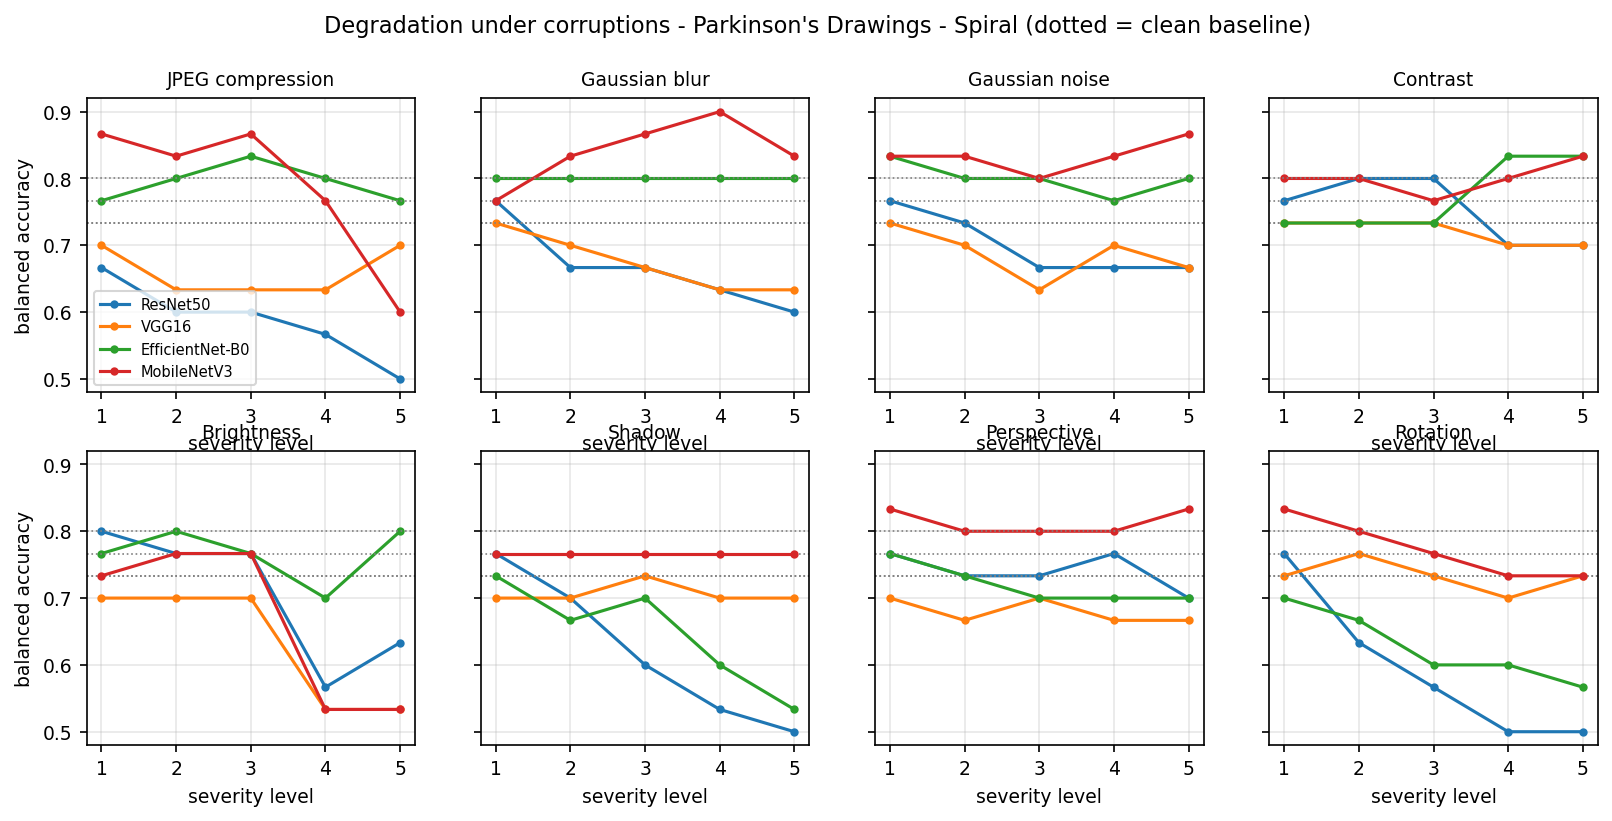
\includegraphics[width=0.98\linewidth]{../../results/figures/fig_curves_pdraw_spiral.png}
\caption{Balanced accuracy versus corruption severity (Parkinson's Drawings,
spiral; dotted lines = clean baseline of each backbone; the remaining three
image types in Figs.~S1--S3).}
\label{fig:curves}
\end{figure}

\subsection{Parkinson Robustness Score}
Table~\ref{tab:robustness} reports the per-family degradation $D_c$
(Eq.~\ref{eq:drop} with the XAI term of Section~\ref{sec:metrics}) and the
aggregate PRS (Eq.~\ref{eq:prs}); Fig.~\ref{fig:prs} visualizes the scores.
PRS spans 82.4--96.2 across the sixteen configurations at the canonical
seed. Under the evaluated
splits and training seed, the highest \emph{observed} PRS is achieved by
MobileNetV3-Large on HandPD--spiral (94.9) and PDRAW--spiral (93.0), by
EfficientNet-B0 on PDRAW--wave (96.2), and by ResNet50 on HandPD--meander
(92.5); EfficientNet-B0 is the least robust on HandPD--meander (82.4).
These values are single-split observations whose across-seed variability is
quantified in Section~\ref{sec:results} (seed aggregation) rather than
definitive rankings. We note two
interpretation cautions that the released breakdown makes transparent:
relative drops are computed against each model's own clean value, so
configurations with lower clean baselines can accumulate smaller relative
losses (a floor effect visible for EfficientNet-B0 on the PDRAW types); and
the XAI term contributes up to 20\% of $D_c$, so a model can trade
prediction stability for explanation stability. Both a plain-accuracy variant
of the score and all components are included in the released CSVs.

\textbf{Weight sensitivity.} Because $(w_1, w_2, w_3)$ is a modelling choice,
we recompute PRS under a performance-only weighting $(0.7, 0.3, 0)$ and an
equal weighting $(1/3, 1/3, 1/3)$ (Table~S3). The model ranking per image
type is identical under the equal weighting (Spearman $\rho = 1.0$ for every
dataset) and near-identical under the performance-only weighting (mean
$\rho = 0.95$; the only deviation is one adjacent swap between VGG16 and
MobileNetV3-Large on HandPD--spiral), so the headline conclusions do not
depend on the chosen weights; absolute scores shift by up to ${\approx}5$
points.

\textbf{Seed variability.} Table~\ref{tab:seeds} reports clean accuracy,
ROC-AUC and PRS as mean\,$\pm$\,standard deviation over the three training
seeds (42/43/44). Comparing across seeds, two effects are visible. First, absolute PRS levels vary by
several points across seeds (standard deviations 0.3--10.5 points), as
expected with 72--260 training images; clean accuracy itself varies by up to
$\pm$17.6 points (VGG16 on PDRAW--wave). Second, ranking stability is
dataset-dependent: pairwise Spearman correlations between per-seed PRS
rankings range from $-0.8$ to $+0.8$ on the small PDRAW splits -- partly a
floor effect, since the $\Delta$ terms are normalized by each model's own
clean baseline, so configurations with lower clean accuracy can accumulate
small relative drops -- versus 0.4--1.0 on HandPD. By mean PRS,
EfficientNet-B0 leads on both PDRAW types, and VGG16 and ResNet50 lead on
one HandPD type each, while MobileNetV3-Large's weak robustness on
HandPD--meander (PRS ${\approx}88$) is consistent across all three seeds.
PRS should therefore be read as a per-protocol observation with
quantifiable uncertainty, not as a deterministic model property.

\begin{table}[t]
\centering\small
\caption{Mean\,$\pm$\,standard deviation over three training seeds
(42/43/44) of clean test accuracy, clean ROC-AUC and PRS.}
\label{tab:seeds}
\begin{tabular}{llccc}
\toprule
Dataset & Model & Accuracy & ROC-AUC & PRS \\
\midrule
HandPD--meander & EffNet-B0 & 0.864±0.027 & 0.834±0.011 & 83.0±1.0 \\
HandPD--meander & MobileNetV3 & 0.815±0.049 & 0.836±0.003 & 88.1±5.3 \\
HandPD--meander & ResNet50 & 0.849±0.014 & 0.862±0.012 & 93.5±1.1 \\
HandPD--meander & VGG16 & 0.880±0.018 & 0.861±0.024 & 92.1±3.1 \\
HandPD--spiral & EffNet-B0 & 0.886±0.037 & 0.981±0.005 & 88.0±0.3 \\
HandPD--spiral & MobileNetV3 & 0.920±0.044 & 0.970±0.022 & 91.8±2.7 \\
HandPD--spiral & ResNet50 & 0.892±0.014 & 0.960±0.014 & 91.0±1.4 \\
HandPD--spiral & VGG16 & 0.907±0.032 & 0.934±0.042 & 93.7±2.0 \\
PDRAW--spiral & EffNet-B0 & 0.722±0.039 & 0.870±0.005 & 93.0±1.7 \\
PDRAW--spiral & MobileNetV3 & 0.811±0.019 & 0.918±0.007 & 89.7±4.3 \\
PDRAW--spiral & ResNet50 & 0.722±0.084 & 0.932±0.009 & 89.1±1.5 \\
PDRAW--spiral & VGG16 & 0.722±0.019 & 0.816±0.011 & 92.3±5.5 \\
PDRAW--wave & EffNet-B0 & 0.778±0.051 & 0.936±0.007 & 94.0±4.4 \\
PDRAW--wave & MobileNetV3 & 0.878±0.069 & 0.942±0.019 & 86.6±3.1 \\
PDRAW--wave & ResNet50 & 0.856±0.051 & 0.917±0.011 & 91.8±1.5 \\
PDRAW--wave & VGG16 & 0.767±0.176 & 0.892±0.019 & 85.8±10.5 \\

\bottomrule
\end{tabular}
\end{table}

\begin{table}[t]
\centering\small
\caption{Per-family weighted degradation $D_c$ and the aggregate Parkinson
Robustness Score (PRS; 0--100, higher = more robust; weights
$w = 0.5/0.3/0.2$ for balanced accuracy, F1, and XAI stability).}
\label{tab:robustness}
\begin{tabular}{llcccccccc}
\toprule
Dataset & Model & JPEG & Blur & Noise & Contr. & Bright. & Shadow & Persp. & Rot. & PRS \\
\midrule
HandPD--meander & ResNet50 & 0.087 & 0.028 & 0.015 & 0.026 & 0.102 & 0.037 & 0.093 & 0.216 & 92.5 \\
HandPD--meander & VGG16 & 0.053 & 0.028 & 0.052 & 0.025 & 0.200 & 0.043 & 0.052 & 0.433 & 88.9 \\
HandPD--meander & MobileNetV3 & 0.141 & 0.138 & 0.166 & 0.012 & 0.152 & 0.047 & 0.176 & 0.405 & 84.5 \\
HandPD--meander & EffNet-B0 & 0.109 & 0.182 & 0.037 & 0.048 & 0.217 & 0.037 & 0.275 & 0.503 & 82.4 \\
HandPD--spiral & MobileNetV3 & 0.021 & 0.014 & 0.003 & 0.011 & 0.093 & 0.100 & 0.070 & 0.096 & 94.9 \\
HandPD--spiral & VGG16 & 0.016 & 0.044 & 0.034 & 0.017 & 0.076 & 0.052 & 0.078 & 0.135 & 94.3 \\
HandPD--spiral & ResNet50 & 0.067 & 0.102 & 0.067 & 0.009 & 0.130 & 0.116 & 0.083 & 0.168 & 90.7 \\
HandPD--spiral & EffNet-B0 & 0.123 & 0.171 & 0.029 & 0.086 & 0.193 & 0.053 & 0.135 & 0.175 & 87.9 \\
PDRAW--spiral & MobileNetV3 & 0.051 & 0.008 & -0.002 & 0.017 & 0.167 & 0.073 & 0.067 & 0.180 & 93.0 \\
PDRAW--spiral & EffNet-B0 & 0.012 & 0.006 & 0.021 & 0.004 & 0.051 & 0.152 & 0.196 & 0.231 & 91.6 \\
PDRAW--spiral & ResNet50 & 0.181 & 0.112 & 0.084 & 0.006 & 0.083 & 0.155 & 0.043 & 0.231 & 88.8 \\
PDRAW--spiral & VGG16 & 0.189 & 0.180 & 0.128 & 0.042 & 0.255 & 0.070 & 0.161 & 0.094 & 86.0 \\
PDRAW--wave & EffNet-B0 & 0.036 & 0.030 & -0.112 & -0.034 & -0.031 & 0.089 & 0.006 & 0.324 & 96.2 \\
PDRAW--wave & ResNet50 & 0.004 & 0.027 & 0.054 & 0.013 & 0.020 & 0.069 & 0.048 & 0.304 & 93.2 \\
PDRAW--wave & VGG16 & 0.098 & 0.120 & 0.098 & 0.083 & 0.143 & 0.049 & 0.130 & 0.217 & 88.3 \\
PDRAW--wave & MobileNetV3 & 0.059 & 0.126 & 0.069 & 0.006 & 0.110 & 0.053 & 0.070 & 0.585 & 86.5 \\

\bottomrule
\end{tabular}
\end{table}

\begin{figure}[t]
\centering
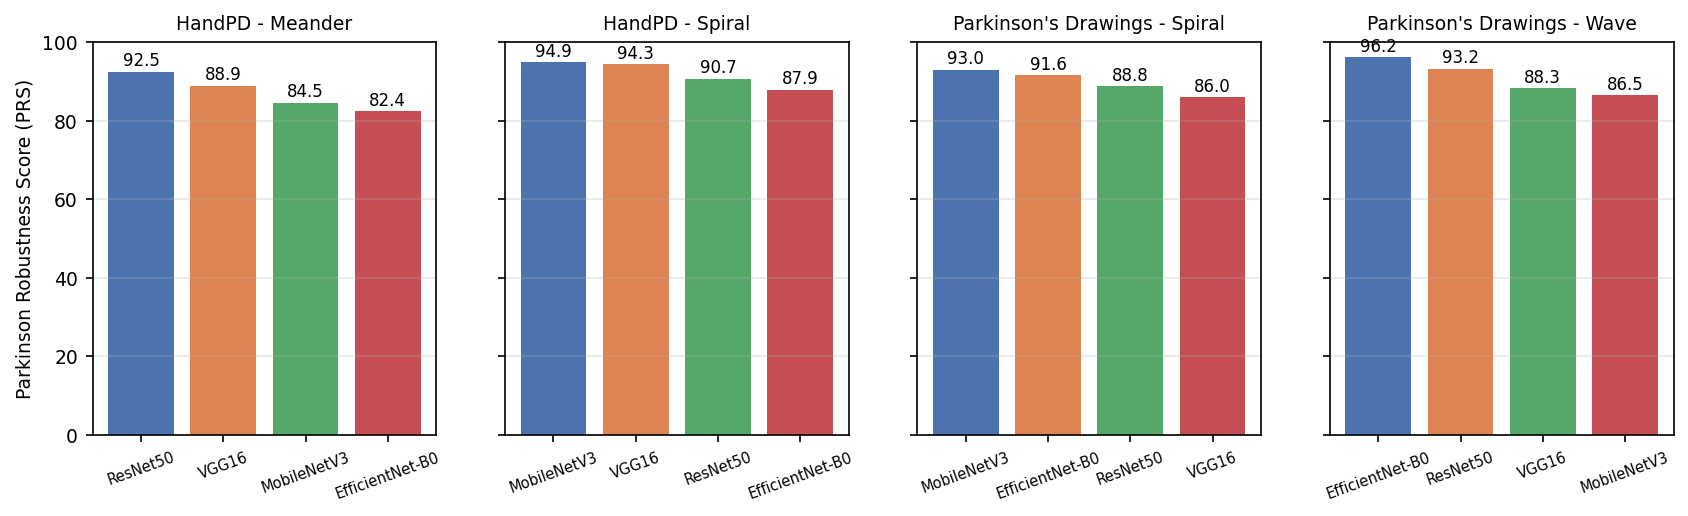
\includegraphics[width=0.98\linewidth]{../../results/figures/fig_robustness_scores.png}
\caption{Parkinson Robustness Score per backbone and image type.}
\label{fig:prs}
\end{figure}

\section{Discussion}
\label{sec:discussion}

\subsection{XAI Analysis}
\label{sec:xai}

\subsubsection{Quantitative stability}
Table~\ref{tab:xai} reports the mean Spearman rank correlation between each
corrupted Grad-CAM map and the corresponding clean map (10 test images per
type: 5 PD, 5 healthy; all severities averaged). The ordering of corruption
families mirrors -- but is \emph{not identical to} -- the accuracy ordering:
rotation is by far the most disruptive to explanations ($\bar\rho = 0.42$,
falling to $\rho = 0.29$ at severity~5), followed by perspective
($\bar\rho = 0.66$), whereas contrast leaves the maps nearly
unchanged ($\bar\rho = 0.92$). JPEG compression, which costs only 4--6\%
balanced accuracy on average, degrades explanation stability substantially
($\rho$ falling from 0.96 at severity~1 to 0.62 at severity~5); the same
severity-wise decay holds for noise (0.96$\rightarrow$0.77), blur
(0.91$\rightarrow$0.73) and brightness (0.79$\rightarrow$0.55), as
visualized in Fig.~\ref{fig:xaistab}. Secondary metrics agree (family-mean
Pearson 0.37--0.95, SSIM 0.52--0.89, and top-20\% IoU 0.30--0.77 across
families, with rotation and contrast at the two extremes).

\begin{table}[t]
\centering\small
\caption{Grad-CAM stability under corruption: mean Spearman correlation of
corrupted vs.\ clean saliency maps (all severities, 10 images per type).}
\label{tab:xai}
\begin{tabular}{llcccccccc}
\toprule
Dataset & Model & JPEG & Blur & Noise & Contr. & Bright. & Shadow & Persp. & Rot. \\
\midrule
HandPD--meander & EffNet-B0 & 0.93 & 0.85 & 0.95 & 0.94 & 0.77 & 0.78 & 0.58 & 0.37 \\
HandPD--meander & MobileNetV3 & 0.89 & 0.90 & 0.87 & 0.94 & 0.77 & 0.89 & 0.71 & 0.49 \\
HandPD--meander & ResNet50 & 0.84 & 0.86 & 0.89 & 0.90 & 0.78 & 0.88 & 0.64 & 0.44 \\
HandPD--meander & VGG16 & 0.90 & 0.89 & 0.92 & 0.90 & 0.80 & 0.89 & 0.78 & 0.55 \\
HandPD--spiral & EffNet-B0 & 0.90 & 0.67 & 0.89 & 0.87 & 0.74 & 0.76 & 0.64 & 0.28 \\
HandPD--spiral & MobileNetV3 & 0.94 & 0.94 & 0.94 & 0.96 & 0.82 & 0.83 & 0.78 & 0.70 \\
HandPD--spiral & ResNet50 & 0.85 & 0.84 & 0.85 & 0.91 & 0.75 & 0.78 & 0.67 & 0.49 \\
HandPD--spiral & VGG16 & 0.91 & 0.89 & 0.90 & 0.93 & 0.72 & 0.79 & 0.72 & 0.50 \\
PDRAW--spiral & EffNet-B0 & 0.79 & 0.81 & 0.77 & 0.93 & 0.74 & 0.70 & 0.22 & 0.38 \\
PDRAW--spiral & MobileNetV3 & 0.72 & 0.74 & 0.80 & 0.92 & 0.72 & 0.86 & 0.63 & 0.34 \\
PDRAW--spiral & ResNet50 & 0.75 & 0.74 & 0.73 & 0.88 & 0.70 & 0.72 & 0.75 & 0.46 \\
PDRAW--spiral & VGG16 & 0.67 & 0.60 & 0.74 & 0.90 & 0.59 & 0.78 & 0.63 & 0.53 \\
PDRAW--wave & EffNet-B0 & 0.91 & 0.89 & 0.90 & 0.94 & 0.81 & 0.87 & 0.61 & 0.34 \\
PDRAW--wave & MobileNetV3 & 0.84 & 0.76 & 0.89 & 0.95 & 0.73 & 0.85 & 0.66 & 0.32 \\
PDRAW--wave & ResNet50 & 0.86 & 0.77 & 0.81 & 0.93 & 0.78 & 0.80 & 0.74 & 0.15 \\
PDRAW--wave & VGG16 & 0.80 & 0.76 & 0.80 & 0.89 & 0.67 & 0.81 & 0.64 & 0.28 \\

\bottomrule
\end{tabular}
\end{table}

\begin{figure}[t]
\centering
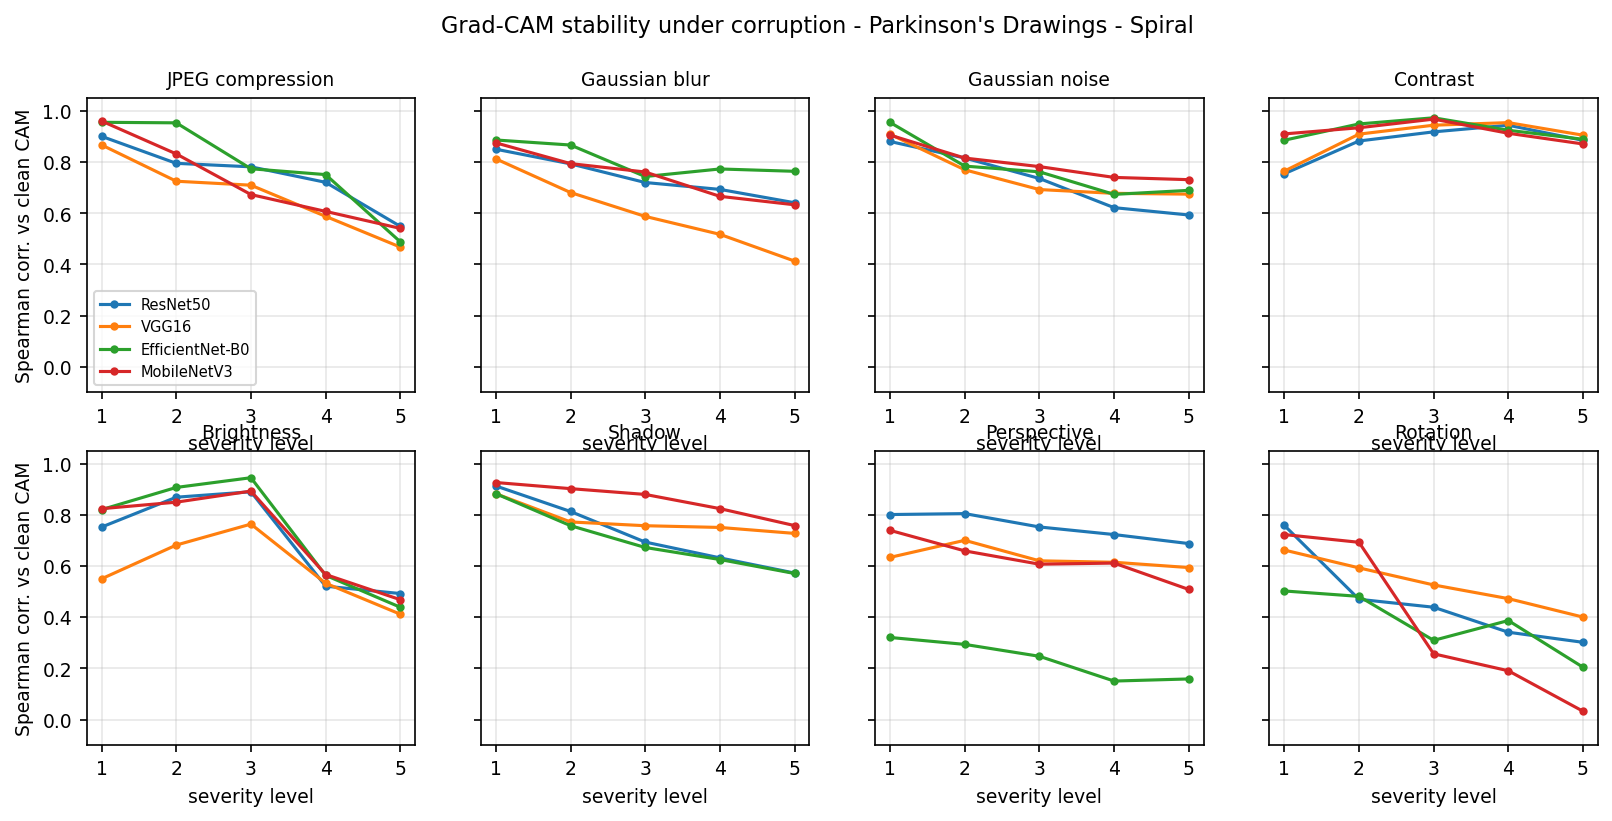
\includegraphics[width=0.98\linewidth]{../../results/figures/fig_xai_stability_pdraw_spiral.png}
\caption{Spearman correlation with the clean Grad-CAM map versus severity
(Parkinson's Drawings, spiral).}
\label{fig:xaistab}
\end{figure}

\subsubsection{Qualitative observations}
Fig.~\ref{fig:gradcam} overlays the PD-class Grad-CAM evidence for one PD and
one healthy test image under the clean condition and three maximum-severity
corruptions. Under mild degradations the attention remains anchored on the
pen trajectory; under severe blur or compression the evidence spreads from
the spiral strokes to the paper background, and under rotation the hotspot
moves to a different region of the drawing altogether. In other words, a
model may output the correct label while localizing it for a different
reason -- a failure mode invisible to accuracy-only evaluation and directly
relevant when such maps are shown to clinicians \cite{adebayo2018}.

\subsubsection{Stability is not validity}
\label{sec:sanity}
A minimal model-randomization control \cite{adebayo2018} supports that the
maps track learned, model-specific evidence rather than acting as
input-only edge detectors: replacing the trained head and fine-tuned stage
with freshly initialized parameters collapses the rank agreement with the
trained models' maps (mean Spearman over the PDRAW-spiral subset: 0.23 for
ResNet50, $-0.15$ for VGG16, 0.04 for EfficientNet-B0, and 0.07 for
MobileNetV3-Large, whose untrained
instance produces constant maps; per-image values released as
\texttt{results/gradcam\_sanity.csv}), whereas the corruption-stability
correlations of the trained models remain high (Table~\ref{tab:xai}).
We nevertheless emphasise that this study measures \emph{explanation
stability} only -- how much a map changes under corruption -- and does not
establish that Grad-CAM maps are faithful or clinically valid descriptions
of the models' reasoning; faithfulness would require additional occlusion or
deletion/insertion tests, which we identify as future work.

\begin{figure}[t]
\centering
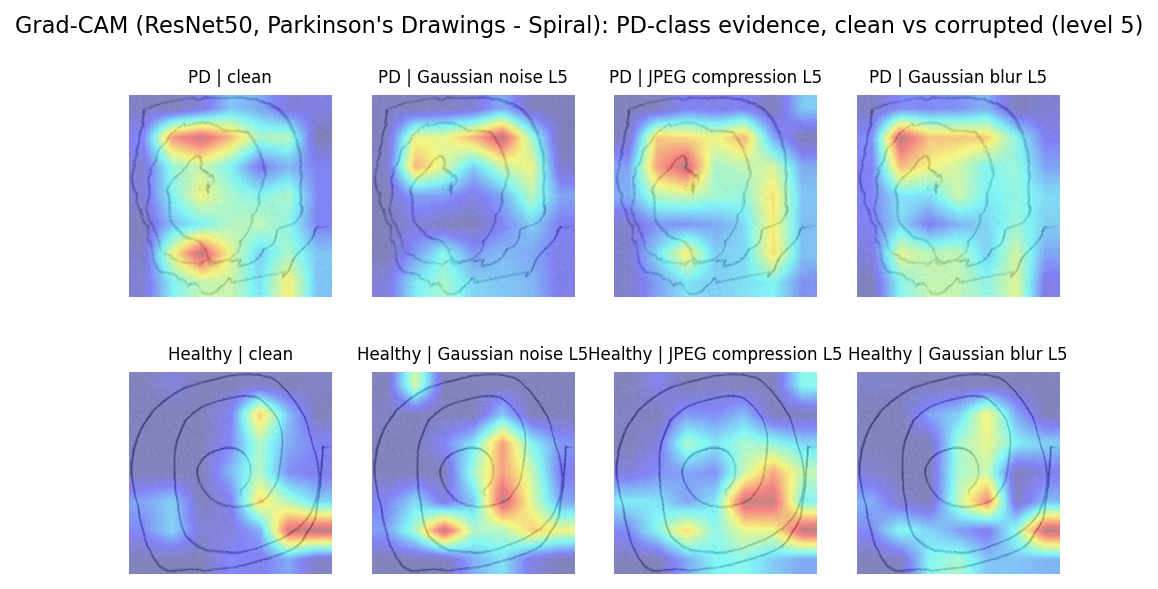
\includegraphics[width=0.9\linewidth]{../../results/figures/fig_gradcam_pdraw_spiral_resnet50.png}
\caption{Grad-CAM overlays (ResNet50, PDRAW spiral): PD-class evidence on a
PD image (top) and a healthy image (bottom), clean vs.\ corrupted at
severity 5.}
\label{fig:gradcam}
\end{figure}


\textbf{What the results mean for practice.} The benchmark shows that
deployed PD-drawing classifiers face their largest risk not from sensor noise
or compression but from \emph{geometric} variation and uneven illumination --
inexpensive, largely controllable factors at acquisition time. Standardizing
sheet orientation and lighting, or including small rotations and illumination
gradients in any training-time augmentation, is likely to remove the largest
degradation sources; our frozen-backbone protocol
keeps this hypothesis testable within the same framework. Second, the
explanation-stability results argue for reporting XAI robustness alongside
accuracy: JPEG compression, the most common real-world degradation of
photographed drawings, leaves predictions almost intact while redrawing the
model's justification.

\textbf{Why a single score, and what it hides.} PRS is deliberately simple,
weighted and decomposable: every number inside it (per family, per metric)
is released, so the scalar serves as an entry point rather than a summary
that obscures failures. The floor-effect caveat of relative drops
(Section~\ref{sec:results}) and the family-specific rankings both argue
against reading PRS without its breakdown.

\textbf{Limitations.} (i) The backbones are adapted with a deliberately light
two-stage protocol (head + last-stage fine-tune) on small training splits;
stronger training recipes would shift clean baselines upward and likely also
shift robustness, although published evidence that augmentation improves
corruption robustness \cite{boone2023} suggests rankings may be preserved.
(ii) Test sets are small (30 images per PDRAW type, 108 per HandPD type), so
per-condition metrics carry non-trivial uncertainty (bootstrap intervals of
up to $\pm$16.7 accuracy points, Section~\ref{sec:results}); we mitigate this
by averaging over severities and families and by releasing per-image
predictions. (iii) Corruptions are \emph{synthetic} approximations inspired
by common acquisition and digitization variations (compression of
photographed drawings, defocused scans, sensor noise, uneven exposure, cast
shadows, non-parallel sheet placement); parameter choices were not calibrated on physically degraded
acquisitions, and external validity against a field-collected degraded set
has not yet been verified. (iv) We evaluate Grad-CAM only; extending the
stability analysis to LIME or integrated gradients is straightforward in the
released code, and faithfulness tests (occlusion, deletion/insertion) remain
future work (Section~\ref{sec:sanity}). (v) Three training seeds are used
per configuration, which quantifies but does not eliminate protocol
variance: with training splits of only 72--260 images, seed-level PRS
varies by several points and PDRAW rankings partially re-order
(Section~\ref{sec:results}), so scores should be read as observations
under this specific protocol rather than as definitive model rankings. (vi) The PDRAW release
provides no subject identifiers, so subject-level independence between its
train and test partitions cannot be verified; any subject overlap would
primarily inflate clean absolute metrics but leaves within-configuration
degradation analyses largely unaffected. Finally, the framework is intended
for methodological benchmarking; it does not establish clinical validity of
any evaluated model.

\textbf{Future work.} Natural extensions include: NewHandPD and PaHaW as
additional datasets; vision-transformer backbones; training-time mitigation
(orientation-aware augmentation, corruption-aware fine-tuning) evaluated
inside the same benchmark; subject-level aggregation of predictions; and
certified-robustness bounds for the geometric family.

\subsection{Conclusion}
\label{sec:conclusion}
We presented PD-RobustBench, a reproducible corruption-robustness and
explainability evaluation framework for deep-learning detection of
Parkinson's disease from hand-drawn images. The benchmark covers two public
datasets and four image types, four ImageNet-pretrained backbones, eight
corruption families at five severity levels, a Grad-CAM stability analysis
with a randomization control, and a decomposable Parkinson Robustness Score
that was evaluated over three training seeds and three weighting schemes.
The benchmark supports three main conclusions. First, geometric misalignment
(rotation) and uneven illumination (shadows) degrade all evaluated backbones
far more than compression or sensor noise; both factors are largely
controllable at acquisition time. Second, explanation maps drift faster than
predictions under common compressions, so accuracy alone conceals a failure
mode that matters whenever saliency maps are shown to clinicians. Third,
backbone rankings depend on the corruption family and are only partially
stable across seeds, which argues for reporting full degradation profiles
with uncertainty rather than single numbers. All code, corruption
definitions, trained heads, per-image predictions, saliency maps and
sensitivity analyses are released, and new backbones can be added through a
three-point registration interface, so the benchmark can grow with the
field.

\section*{Data and code availability}
The complete framework is released, including: the corruption benchmark
specification (\texttt{docs/task3\_1\_corruption\_levels.csv}); all
evaluation and analysis scripts (\texttt{src/}); trained model heads and
decision thresholds (\texttt{checkpoints/}, \texttt{results/thresholds.csv});
per-image predictions for every model $\times$ corruption $\times$ severity
condition (\texttt{results/predictions.csv}); bootstrap confidence intervals
(\texttt{results/bootstrap\_ci.csv}); the PRS decomposition and weight
sensitivity analysis (\texttt{results/robustness\_breakdown.csv},
\texttt{results/prs\_sensitivity.csv}); the three-seed aggregation
(\texttt{results/seed\_aggregate.csv}); saved Grad-CAM maps
(\texttt{xai\_outputs/}) and the randomization control
(\texttt{results/gradcam\_sanity.csv}); and all figures and tables. Code:
\url{[REPOSITORY-URL]}. Datasets: Parkinson's Drawings (Kaggle release
\cite{kagglepdrawings}) and HandPD \cite{handpddata,pereira2016}.

\section*{Conflict of interest}
The authors declare no conflict of interest.

%----------------------------------------------------------------------
\begin{thebibliography}{99}\small

\bibitem{zham2016} P.~Zham, S.~P.~Arjunan, S.~Raghav, D.~K.~Kumar,
``Efficacy of guided spiral drawing in the classification of Parkinson's
disease,'' \emph{IEEE EMBC}, pp.~5007--5010, 2016.

\bibitem{zham2017} P.~Zham, S.~P.~Arjunan, S.~Raghav, D.~K.~Kumar,
``Distinguishing different stages of Parkinson's disease using composite
index of speed and pen-pressure of sketching a spiral,'' \emph{Frontiers in
Neurology}, 8:435, 2017.

\bibitem{pereira2016} C.~R.~Pereira et al., ``A new computer vision-based
approach to aid the diagnosis of Parkinson's disease,'' \emph{Computer
Methods and Programs in Biomedicine}, 136:79--88, 2016.

\bibitem{huang2024} Y.~Huang et al., ``Early Parkinson's disease diagnosis
through hand-drawn spiral and wave analysis using deep learning
techniques,'' \emph{Information}, 15(4):220, 2024.

\bibitem{frontiers2024} ``Utilizing deep learning models in an intelligent
spiral drawing classification system,'' \emph{Frontiers in Medicine},
11:1453743, 2024.

\bibitem{aims2024} ``Modeling and diagnosis Parkinson disease by using hand
drawing,'' \emph{AIMS Mathematics}, 9(10):28012--28037, 2024.

\bibitem{diagnostics2025} A.~Razaq et al., ``Deep learning framework for
early PD detection,'' \emph{Diagnostics}, 15(21):2795, 2025.

\bibitem{ml4h2021} ``Machine learning for real-time, automatic, and early
diagnosis of Parkinson's disease by extracting signs of micrographia from
handwriting images,'' \emph{ML4H Workshop}, 2021 (arXiv:2111.14781).

\bibitem{hendrycks2019} D.~Hendrycks, T.~Dietterich, ``Benchmarking neural
network robustness to common corruptions and perturbations,'' \emph{ICLR},
2019 (arXiv:1903.12261).

\bibitem{croce2021} F.~Croce et al., ``RobustBench: a standardized
adversarial robustness benchmark,'' \emph{LDMI}, 2021.

\bibitem{medmnistc} R.~Herde et al., ``MedMNIST-C: 12 corrupted benchmark
datasets and augmentation APIs for robust medical image classification,''
Univ.\ Bamberg, 2024.

\bibitem{boone2023} L.~Boone et al., ``ROOD-MRI: benchmarking the robustness
of deep learning segmentation networks to distribution shift,'' \emph{NeuroImage}, 280:120920, 2023.

\bibitem{javed2024} H.~Javed et al., ``Robustness in deep learning models for
medical diagnostics: a survey,'' \emph{Artificial Intelligence Review}, 57,
2024.

\bibitem{shen2025} X.~Shen et al., ``Improving robustness and reliability in
medical image classification,'' 2025 (PubMed 40587343).

\bibitem{selvaraju2017} R.~R.~Selvaraju et al., ``Grad-CAM: visual
explanations from deep networks via gradient-based localization,''
\emph{ICCV}, pp.~618--626, 2017.

\bibitem{adebayo2018} J.~Adebayo et al., ``Sanity checks for saliency
maps,'' \emph{NeurIPS}, pp.~9505--9515, 2018.

\bibitem{resnet} K.~He, X.~Zhang, S.~Ren, J.~Sun, ``Deep residual learning
for image recognition,'' \emph{CVPR}, pp.~770--778, 2016.

\bibitem{vgg} K.~Simonyan, A.~Zisserman, ``Very deep convolutional networks
for large-scale image recognition,'' \emph{ICLR}, 2015.

\bibitem{efficientnet} M.~Tan, Q.~Le, ``EfficientNet: rethinking model
scaling for convolutional neural networks,'' \emph{ICML}, 2019.

\bibitem{mobilenetv3} A.~Howard, M.~Sandler, et al., ``Searching for
MobileNetV3,'' \emph{ICCV}, pp.~1314--1324, 2019 (arXiv:1905.02244).

\bibitem{kagglepdrawings} K.~S.~Mader, ``Parkinson's Drawings,'' Kaggle
dataset, \url{https://www.kaggle.com/datasets/kmader/parkinsons-drawings}.

\bibitem{handpddata} J.~P.~Papa lab, ``HandPD dataset,''
\url{https://wwwp.fc.unesp.br/~papa/pub/datasets/Handpd/}.

\end{thebibliography}

\end{document}
